\documentclass[conference]{IEEEtran}
\usepackage{cite}
\usepackage{graphicx}
\usepackage{algorithm2e}

% Judul
\title{Implementasi Algoritma Dijkstra Dalam
Menemukan Jarak Terdekat}

% Penulis
\author{\IEEEauthorblockN{Reynaldo A. A. Putra}
\IEEEauthorblockA{\textit{School of Electrical Engineering and Informatics}\\
\textit{Institut Teknologi Bandung}\\
Bandung, Indonesia\\
Email: NIM@std.stei.itb.ac.id}
}

\graphicspath{.\gambar}

\begin{document}

\maketitle

\begin{abstract}
    Kebun Raya Purwodadi dengan luas area sekitar 85
hektar ternyata kekurangan papan informasi yang menyebabkan
pengunjung kerap kali kebingungan dalam mencari lokasi tanaman tertentu. Integer fringilla luctus quam eget commodo. Donec sapien nibh, tristique eu metus placerat, fringilla vestibulum purus. Pellentesque turpis ligula, convallis nec volutpat non, mollis ut erat. Cras id placerat arcu. Nullam bibendum odio at lobortis consequat. Proin in elit neque. Duis vestibulum velit in leo iaculis interdum. Duis vulputate sem nunc, non rutrum dolor dignissim at. Nam laoreet elit odio, ut dictum felis dapibus eu. Praesent augue nisl, iaculis nec urna id, ultrices dignissim leo. Vivamus velit metus, hendrerit id aliquet ac, porta non nisl.    
\end{abstract}

\begin{IEEEkeywords}
    Dijkstra, Vertex, Edge, Tanaman.
\end{IEEEkeywords}

\section{Pembuka}
Lorem ipsum dolor sit amet, consectetur adipiscing elit. Sed tristique iaculis massa, et lacinia ipsum dapibus eget. Nam non convallis dui. In eleifend ante scelerisque convallis imperdiet. Sed tempus est vehicula finibus posuere. In ut massa magna. Aenean suscipit, velit id eleifend ullamcorper, turpis nibh sagittis elit, sed vehicula augue sem id mauris. Aenean sed nulla malesuada ipsum congue consequat vitae ut magna. Fusce sed laoreet nulla.

\subsection{Algoritma Dijkstra}
Algoritma Dijkstra adalah algoritma yang digunakan untuk
menemukan jarak jalur terpendek antara dua vertice pada
graph berbobot dan tidak berarah sederhana \cite{he2022application}

\SetKwComment{Comment}{/* }{ */}
\RestyleAlgo{ruled}

\begin{algorithm}
    \caption{: Fungsi Graph \texttt{(printgraph)}}\label{alg:one}
    \RestyleAlgo{ruled}
\KwResult{ Memunculkan Graph $n \times n$ Ke Layar}
\textbf{procedure}  $printgraph(n, graph[n][n])$\;
\While{$i \leq n-1$}{
    $j \gets 0$\;
    \While{$j \leq n-1$}{
        \eIf{$graph [i][j] = int_max$}{
            \textbf{output:} (-1)\;
        }{
            \textbf{output:} ($graph[n][n]$)\;
        }
        $j \gets j + 1$\;
    }
    $i \gets i + 1$\;
}
\end{algorithm}
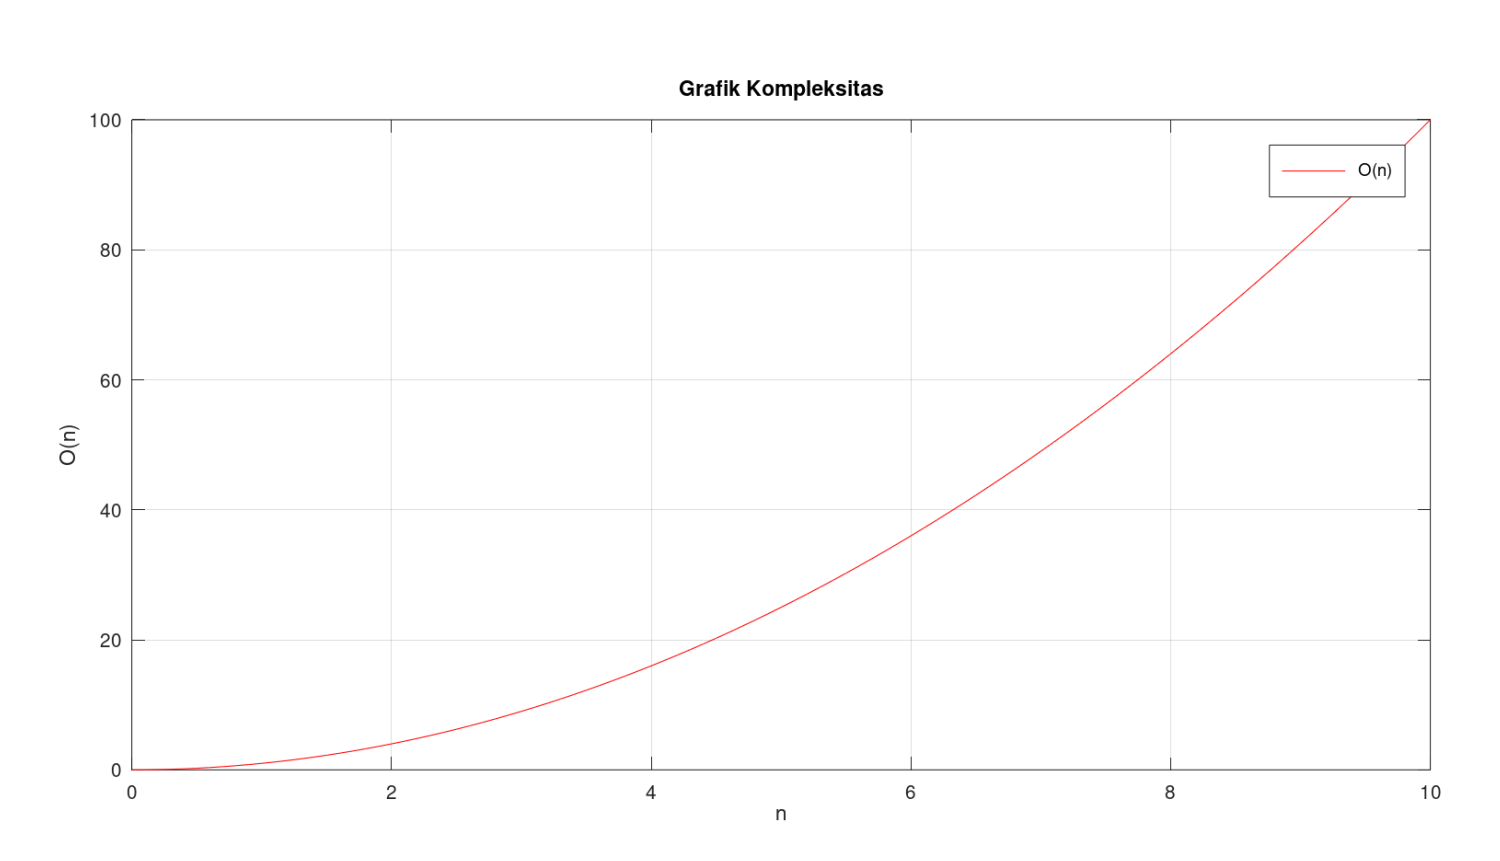
\includegraphics[width=0.5\textwidth]{gambar/graph.png}
\bibliographystyle{IEEEtran}
\bibliography{references.bib}

\end{document}